\chapter{Gamemaster Tools}
\label{ch:more-rules-advice}

Gamemasters typically need to know more rules than the players. They need to handle situations that go beyond a single character, like doing mass battles or travelling by ships, optional creature plunder, etc. This chapter consolidates such rules for the benefit of Gamemasters.


\section{Plunder Rating}

Although Fantasy D100 is not a game of ‘Killing Things and Taking their Stuff’, it is sometimes useful and expected that creatures that the Player Characters meet upon their Quests will have treasure, both mundane and magical.

Normally the needs of the story can dictate what treasure and supernatural items a creature possesses, but if a quick random roll is necessary the following guidelines can be consulted.

Each creature has a Plunder Rating which is a rating of how much treasure the creature is likely to be carrying. For creatures that form groups, increase the Plunder Rating by at least one, for groups of up to 20 creatures, by two for larger groups of up to a hundred creatures, and by 3 for groups of over a hundred. In this case the Plunder will be held in a defended and guarded treasure room which the leader of the creatures will have access to.

The following table has a list of potential treasure for creatures depending on their Plunder Rating. If applicable (e.g. campaign has supernatural Disciplines, like magic) also roll for the supernatural items.

\begin{table}
\begin{center}
\caption{Plunder}
\label{tab:plunder}
\begin{rpg-table}[|c|X|]
	\hline
        \textbf{Plunder Rating}  & \textbf{Treasure Found}\\
        \hline
	0 & Not a hoarder. No treasure whatsoever.\\
        1 & Chance hoarder. A couple of coppers, loose change (1D6 CPs). Very remote (05\%) chance of a supernatural item, which is either used by accident (my lucky talisman) or which the creature is completely oblivious to.\\
	2 & Hoards enough for a rainy day. About 5D20 in SPs, 1D10 GPs. If the creature has supernatural abilities, there is a POW \% chance of 1D4 Minor supernatural items appropriate to the type.\\
	3 & Hoards for a better future. Collects treasure for its worth and appreciates its value. 5D100 in SPs, 3D20 in GPs. If the creature has supernatural abilities, there is a POW X 2\% chance of 1D4 appropriate Minor supernatural items.\\
	4 & Significant hoard. Hoards for hoarding’s sake. 10D100 SPs, 1D100 GPs. POW X 3\% of 1D6 Minor supernatural items and POW \% chance of 1D4 Major supernatural items.\\
	5 & Treasure trove. The wealth of a minor Lord. Examples: Grave goods of a dead noble worth about 1D6 thousand Silver Pieces, with 1D6 Minor supernatural Items and POW X 3\% chance of 1D6 Major supernatural Items.\\
	6 & Wealth of Kings. eg. Dragon’s Hoard, a hoard almost beyond comprehension 1D4 Million Silver pieces, 2D10 Minor, 1D8 Major and one unique supernatural item.\\
	\hline
\end{rpg-table}
\end{center}
\end{table}


\section{Ships and Sailing}

\subsection{Construction}
There are, broadly speaking, three types of sailing ship: sloops (small, fast, but comparatively fragile one-masted vessels), brigs (fast and manoeuvrable two-masted vessels), and ships (larger vessels with at least three masts, whether warships or cargo vessels).

Weapons are handled abstractly; ship-mounted weapons are not accurate, and large numbers of shots are fired in order to have a chance to hit an enemy ship. Thus a ship’s weapons are rated abstractly as a single percentage chance to hit an enemy vessel in combat; almost certainly many weapons are fired for each “hit roll”. A hit generally does D8 damage, subtracted from the other ship’s structure points.

Every 10\% in weapons reduces cargo capacity by 2 tons, and means two extra crew are needed. The weapons level cannot be increased above 100\%.

Even beyond weapons carried, not all ships are identical; any ship will have one of the following special features.  It might have more than one such feature; in this case, add +50\% of the original cost to the total cost per feature added.

\begin{description}
\item[Armored:] AP 2 against any attacks.
\item[Fast:] Add +1 knot to speed.
\item[Heavy Weapons:] Hits from weapons do D12 rather then D8 damage.
\item[High Capacity:] Increase the cargo size by +40\%.
\item[Manoeuvrable:] Add +20\% to manoeuvrability.
\item[Marines:] The ship can carry (and provide board and lodging for) a number of marines equal to the size of its crew.
\item[Ram:] The ship can ram other vessels in combat without suffering damage.
\item[Reduced Crew:] The crew size needed to run the ship (as indicated table~\ref{tab:ship-types}) is halved.
\end{description}

\begin{table*}
\begin{center}
\caption{Ship Types}
\label{tab:ship-types}
\begin{rpg-table}[|l|Y|Y|c|Y|Y|c|Y|]
	\hline
	\textbf{Type of Ship}  & \textbf{Crew} & \textbf{Cost (SP)} & \textbf{Manoeuvrability} & \textbf{Speed} & \textbf{Structure Points} & \textbf{Cargo} \\
        \hline
	One-masted & 10 & 5000 & +20\% & 6 Knots & 20 & 8 Tons\\
	Two-masted & 20 & 15000 & - & 5 Knots & 40 & 15 Tons\\
	Three-masted & 30 & 50000 & -20\% & 4 Knots & 60 & 30 Tons\\
	\hline
\end{rpg-table}
\end{center}
\end{table*}


\subsection{Sailing Tests}
Most potential manoeuvres a vessel can make are governed by the captain’s Sailing skill, modified by the manoeuvrability of the vessel. A further modifier is the average Sailing skill level of the crew:
\begin{table}[H]
\begin{center}
\begin{rpg-table}[|X|Y|]
        \hline
	25\% or less (no idea) & -20\%\\
	26\%-50\% (competent) & -\\
	51\%-75\% (veteran) & +20\%\\
	76\% or more (expert) & +40\%\\
	\hline
\end{rpg-table}
\end{center}
\end{table}


\subsection{Travel}
In normal sailing conditions, a sailing vessel can move 20 miles per day per knot of speed. Speeds given are averages. Very  favourable  conditions – for example a  good  strong wind in the desired direction of travel (possibly magically arranged) – can double these speeds. As can a rowing crew who critical their Rowing skill test. 

On the other hand, if a ship is becalmed, with no wind at all, it cannot move.

Every day out of sight of land there is a 5\% chance of a storm. Storms do 2D6 structure points of damage to a ship; a ship reduced to zero structure points begins to sink (and will sink almost instantly if its structure points are reduced to the negative of the original amount). Further, sailors on deck must make Dodge tests to stay on board; a sailor swept overboard and not immediately rescued must make an Athletics test to survive.

Fortunately, the captain can make a Sailing test (modified by manoeuvrability) to halve damage from a storm. Better yet, it is possible to plot a course to avoid an incoming storm if it is detected in time (perhaps using magic or skills such as Natural Lore).

\subsection{Naval Combat}
We consider two ranges of distance between ships.

\subsubsection{Contact}
The vessels can see each other. If both vessels wish to close to combat range, or leave contact, this action is of course automatic, and takes about an hour.

If the vessels want different things, roll opposed Sailing tests, as above.

\subsubsection{Combat Range}
Combat between ships is similar to normal combat. Initiative is decided for each ship, rather than between individuals, by saying that the vessel with the better speed goes first.  

A single test is made to fire a ship’s weapons; no defence roll is made against these attacks. If desired, a character can be appointed weapons officer; he oversees the firing of a ship’s weapons.  That character should make a Ranged Combat skill test; if the test succeeds, the ship’s weapons test has a +20\% bonus.

Hand-held weapons are too small to have any effect on an opposing ship, but can be used against those on the decks. Fire is the exception to this rule, being used to set flamable objects, such as decks, and sails, on fire.

The following special manoeuvres can be made by a ship in combat range. One manoeuvre is allowed per round. Each manoeuvre needs a Sailing skill test by the captain, as indicated above.

\subsubsection{Broadside}
If the skill test succeeds, two attacks with a ship’s weapons can be made instead of one.


\subsubsection{Evade}
If the Sailing test succeeds, the opponent cannot use the broadside, ram, or boarding manoeuvres. Further, the vessel can escape combat range (out to contact range) if the other vessel allows it or the Sailing test succeeds as an opposed roll.


\subsubsection{Ram}
The other vessel is rammed if an opposed Sailing test succeeds. A ramming attack does D6 points of damage per mast. If the ship performing this manoeuvre lacks a battering ram, it also takes half the damage inflicted.


\subsubsection{Boarding}
Boarding is possible if an opposed Sailing test succeeds. In this case, the vessels are roped together, and boarding can commence. A free boarding test is allowed immediately after a successful ramming manoeuvre if desired.

If both vessels want to board the other, this is automatic.


%\section{Major Mental Damage}
%This optional rule is best used for Dark Fantasy games, where the tropes of Fantasy are blended with those of Horror. A setting where the characters are Vampire Hunters confronting the dark masters of the night and their minions is a good example of such a game. 

%When characters witness horrific events, the Gamemaster will ask the players to make a Persistence test. Should that fail, then the character has suffered a mental blow so severe their persona has become altered by it. Roll on the Mental Damage Table below to see what kind of effect that the character suffers from. 

%Independent of whether the Persistence test was successful, they must immediately make a Resilience test with a -40\% modifier, or go into shock for 1D4 rounds. 

%\begin{table*}
%\begin{center}
%\caption{Mental Damage Table}
%\label{tab:mental-damage}
%\begin{rpg-table}[|l|X|]
%	\hline
%	\textbf{Roll 1D6}  & \textbf{Effect}\\
%        \hline
%	1 & The shakes – the incident has left you with an uncontrollable but slight and permanent jittery shake. Lose 2 DEX.\\
%	2 & Dislocation – you find it hard to connect with people, it seems easier to remain unfeeling, to simply let things wash right over you. CHA is reduced by 2.\\
%	3 & Losing your rag – suddenly everything and everyone around you is a constant sign of irritation. This irritation you find is best expressed through physical violence. Each time such a situation arises, you must make a Persistence test. Pass and you’ve controlled your rage, fail and you have no recourse but to lash out – either with your fists or any weapons you are carrying.\\
%	4 & Bottling it – when finding yourself in dangerous and stressful situations you have an overwhelming urge to flee, to find safety. Each time such a situation arises, you must make a Persistence test. Pass and you’ve controlled your urge to run, fail and you’ve bottled it totally. \\
%	5 & Nightmares – every night they invade your dreams, forcing you to relive over and over again the things you have witnessed. Sleep becomes almost impossible, a curse rather than a blessing.  CON is reduced by 2.\\
%	6 & Focus – You find yourself having difficulty focusing on the task in hand. Just keeping aware is a struggle. Both POW and INT are reduced by 2.\\
%	\hline
%\end{rpg-table}
%\end{center}
%\end{table*}

%\begin{rpg-examplebox}
%Rurik is helping search a darkened defiled chapel after the party have defeated a group of Ghouls who had taken up residence there. He picks up some sacks that had been left in a corner of the room.  The humidity and heat have done their work on the contents of these bags, turning the contents inside largely to mush. As Rurik lifts the bags, he can feel something solid moving about in that fluid, and realises with a shock that it contains the half-rotten remains for his cousin's head. The Gamemaster rules that this is such a horrific realisation that Rurik must make a Persistence Roll.  

%Rurik has 34\% Persistence. He rolls 51 – a fail. Rurik has been mentally scared by this revelation. He now rolls 1D6 on the Mental Damage Table. He rolls a 5 – from now on his sleep will be plagued by the memory of this instant.  

%Rurik then rolls against his Resilience of 32\%.  He rolls 23 so doesn’t go into shock.  
%\end{rpg-examplebox}

%\subsection{Modifying the Persistence Roll}
%Some monsters are by their very nature more horrific and disturbing than the standard Ghoul or Zombie, such as Greater Demons, Vampire Lords and indescribable monsters of Cosmic Horror. When encountering such leviathans of terror, whose very existence saps the blood from the character’s skin, the Gamemaster may apply a -20\% or even in very rare world threatening circumstances a -40\% modifier to the Persistence Roll.


%\subsection{Spending Hero Points}
%Just as in a Major Wound, characters can spend a Hero Point to avoid the mental damage they would otherwise have incurred. Instead, the character goes into Shock for 1D4 rounds.


%\subsection{Fumbling and Criticals}
%Should your character fumble the Persistence test, then not only do they receive a mental blow but they also go into shock for 1D8 rounds with no chance of a Resilience roll test to avoid.

%Should a character get a critical Persistence, then they have simply shrugged off what has happened and carry on as normal, so a Resilience roll is not required. 


%\subsection{Going into Shock}
%The character becomes numb and unresponsive, can take no further action in combat situations, and can in certain circumstances become a sitting duck. 


\section{Mass Combat}
The following rules can be used if you want a one roll solution to a battle.

Mass combat involves the commanders’ skills of the two opposing sides, modified by the armies involved. The command skills involved are Lore (Military Tactics), and either Influence or Performance.

The actual battle is resolved by opposed Lore (Military Tactics) tests made by the leaders. A successful test means a force inflicts casualties equal to half its size on the opposition. Half of these casualties are deaths; the other half are injuries. These numbers are doubled on a critical success.

Further, the commander of a losing side in a battle must make an Influence or Performance test to prevent a rout. Routing troops either flee in panic, or surrender when they cannot flee. A further 10\% of an army’s numbers are lost in a rout. A critical success on the Influence or Performance test is needed for a force to continue fighting rather than retreating in a more orderly manner. If a force has nowhere to retreat to, it can continue to fight.

The Lore (Military Tactics) test is modified by various situational factors:
\begin{rpg-list}
\item Better equipped than enemy: +20\% bonus.
\item Better trained than enemy: +20\% bonus.
\item Has significant special forces (e.g. artillery, cavalry, combat mages) that the enemy lacks: +20\% bonus for each.
\item Outnumber enemy by two to one or more: +20\% bonus.
\item Outnumber enemy by four to one or more: +40\% bonus.
\item Enemy in defensive position: -20\% penalty.
\item Enemy fortifications: -40\% penalty.
\item Player character heroics (eg: taking out significant enemy, capturing strategic position): +20\% bonus, or -20\% penalty if attempted heroics go horribly wrong.
\end{rpg-list}

Larger forces might split into several armies, each with their own commander. The rules are still as above, but each army must pick another force to attack.


%\section{Hero Points for Plot Edits}
%In Fantasy D100 it is usually the Gamemaster who describes the situation the player characters find themselves in and the outcome of any skill test. This optional rule allows the player to take control of the narrative and change the direction that the story is going in by spending Hero Points. 
%\begin{description}
%\item[1 point for a minor edit:] changes small details in favour of the player. For example, the player character suddenly has an important item of equipment that they previously forgot to bring with them on the quest, or the guard forgets to lock the door to the dungeon that the characters are imprisoned in.
%\item[2 points for a major edit:] puts the player character at an advantage. For example, not only is the dungeon door open but the jail guard is asleep at his table.
%\item[3 points for a drastic edit:] something dramatic and almost impossible happens to put the player character at a major advantage. For example, the king trips up on his flowing robes and, as he falls over, he brings down the three bodyguards who are standing close by, giving the player character assassin a clear bow shot at the tyrant.
%\item[5 points for an implausible edit:] the player stretches the boundaries of plausibility (even within a fantasy setting), to advantage. For example, a passing dragon swoops down and attacks the castle the player characters are imprisoned in, allowing them to escape as the guards are busy fighting off the flying fire-breathing reptile.
%\end{description}
%Plot edits must always come with sensible narration from the player so that even with the five point implausible edit must not break the group’s suspension of disbelief. The Gamemaster has the final say on whether a plot edit is allowed or not.

%Players should not rely on plot edits to constantly overcome obstacles, but save them for moments where they are truly stuck or have a cool situation in mind.

%Plot edits may never completely remove obstacles such as opposing characters or imposing physical challenges, but they can be used to temporarily give players the upper hand. For example you can’t use a plot edit to remove a mountain range or instantly kill a major recurring villain, but you can use one to have your player character find an obscure mountain pass or have the villain temporarily knocked unconscious.

\begin{figure*}
\begin{center}
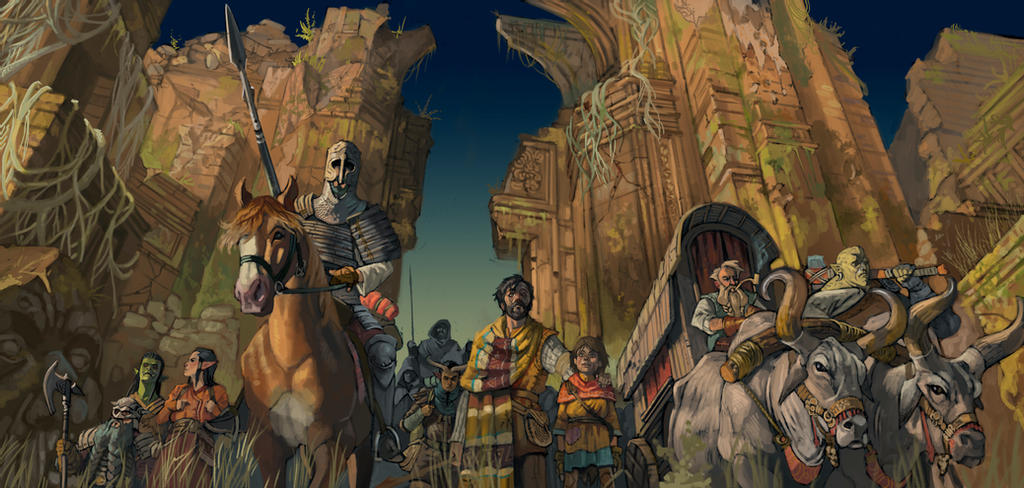
\includegraphics[scale=0.5]{img/settlers_of_the_fallen_city_by_ncorva.jpg}
\end{center}
\end{figure*}



\section{Skill Tests}

\subsection{When to Test}
When the outcome of the character’s action is in doubt or they want to push themselves beyond their expected capacity. If it’s not clear that a character can perform a task, then Gamemaster is well within their rights to call for a skill test.

When it is dramatically appropriate and raises tension in the game. Think carefully before asking for a skill test. Skill tests should be like those moments in a thriller where you are on the edge of your seat and the story could go either way. If the overall result of asking for a skill test is that it will provide the player a success of minor import, such as a minor scrap of information on a Lore roll, just give the player the success without asking them to roll. If the situation is more life or death, describe it as such, highlighting the tension, and ask for a skill test. Where there are definite consequences to a failed skill test, such as falling down a pit filled with spikes if an Athletics skill test is failed, the player should be warned before the character risks taking the action.

\subsection{When not to Test}
As a replacement for good story telling and roleplaying. If the game is flowing nicely as a result of the players and Gamemaster engaging in conversation and weaving a strong exciting story which is keeping everyone happy and entertained through roleplaying, then think twice about breaking that mood by asking for a skill test.

Simply to provide drama and tension in game. The Gamemaster should never substitute a good description of the scene that the players find themselves in, for a series of dice rolls.  

If a similar skill test has just been made. It is tempting to ask for a series of skill tests to simulate a difficult or arduous task, such as climbing an especially difficult cliff, or tracking an opponent through a dense jungle. Don’t. All this does is break player immersion in the game, creating frustration and boredom as several meaningless rolls are made. Instead, ask for a single skill test and modify it to reflect the difficulty of the task. Do not ask for another until the circumstances significantly change.

%\subsection{Creating New Skills}
%Although the Fantasy D100 skill list has been designed to be as concise and complete as possible, during play or during the design of non-player characters for Quests, there may arise a desire to create new skills to describe a previously undiscovered ability. Before introducing a new skill, either by Gamemaster design or player request, consider these two points.

%Is this skill really meaningful and distinct in its own right? Or is it something that can be included in an existing skill?


\section{Fantasy Races}
Most fantasy campaigns will have exotic races as Player Character options. The exact nature of these races will depend on the campaign itself, e.g. Elves in the Tolkien saga are quite different than Elves in the Greyhawk campaign setting.

The Creatures chapter introduction (page~\pageref{ch:creatures}) explains how any creature could be used as a base to create Player Characters. However, a lot of them would not be balanced and the Gamemaster needs to be careful on what races will be allowed in the campaign.

However, some races like Elves, Dwarves or Lizardmen are quite straightforward. Note that when those races have special abilities (e.g. Elves have Night Vision and are Exceptional Archers) they have to spend some of their initial Improvement Points to get that race. That would keep it more balanced for Human characters. Gamemasters have the final say as usual. The following sections contain Elves and Dwarves as examples. 

\subsection{Elves}
The creature entry for Elves (page~\pageref{creature:elf}) has their average Characteristics as well as the dice rolled for the Random Characteristics method. For the point method the starting Characteristics will be analogous to their dice. For example: STR 6, CON 8, DEX 10, SIZ 6, INT 10, POW 8 and CHA 8. Players would then allocate 30 points on top of that.

Remember that the racial top is the maximum possible value plus 3. Thus, Elves can reach a maximum of DEX 27 but only STR 18.

Finally, in their abilities block Elves have Night Sight and are Exceptional Archers. These are useful abilities that would cost 3 Improvement Points each and thus Elf characters will have no extra Improvement Points available during creation.

\subsection{Dwarves}
The creature entry for Dwarves (page~\pageref{creature:dwarf}) has their average Characteristics as well as the dice rolled for the Random Characteristics method. For the point method the starting Characteristics will be analogous to their dice. For example: STR 8, CON 14, DEX 6, SIZ 4, INT 8, POW 8 and CHA 8. Players would then allocate 30 points on top of that.

Remember that the racial top is the maximum possible value plus 3. Thus, Dwarves can reach a maximum of STR and CON of 27.

Finally, in their abilities block Dwarves have Thermoception and Earth Sense. Thermoception is pretty powerful so the player would need to spend 4 Improvement Points to get it. Earch Sense is situational and 2 Improvement Points would be required. Thus Dwarf characters will have no extra Improvement Points available during creation.



\section{Player Archetypes}

The rules allow for an incredible variety of player character concepts. Everything a player can think can be accommodated with the provided rules. To this end, common magic (see chapter~\ref{ch:magic}) can be used to emulate new abilities as supernatural feats rather than consider them as Magic (since some players will not want to use Magic as it conflicts with their character's concept). In this section we provide one such example by describing how a Monk character could be designed.

\subsection{Concept: Monk}
Characters trained in the monastic traditions will be able to achieve some supernatural feats. These characters will go through extensive training to learn special techiques to represent what they have learned in the monastery.

\subsubsection{Rules}
The Player can, of course, use the Battle discipline to improve his fighting abilities but to emulate some of the special monk abilities we can use the Magic discipline. The Player needs to pay Improvement Points to get the Magic discipline and then pay IPs for each Magnitude of spells he is learning. The rules and maximum Magnitude they can learn is exactly as the Magic discipline. The Player character will not be casting spells but all the effects of spell casting need to be emulated. For example it should be obvious for anyone that is seeing the Monk that he is initiating something and under duress they may not succeed.

Flavour is important, so the abilities can be named accordingly. For example, the Player could pay to get the `Monastic' discipline and then learn individual monastic `feats'. Achieving a specific feat requires intense focus and meditation and sometimes distractions might cause failure (explaining why the `Monastic' or `Ki Focus' skill check is required).

\subsubsection{Feats}
The following example feats (spells) can be learned from the monastery: Coordination, Cover Blind Side, Cushion Fall, Extra Defense, Fist of the Wind, Flying Kick, Heal, Ironmind, Leap, Mobility, Multi Attack, Resist (Element), Spirit Shield, Strength, and Weapon Enhance.

Note, however, that they can only be applied to `self' and never to others.


%\subsection{Concept: Druid}

%\subsection{Concept: Elementalist}


\section{Traits, Talents, Feats}

Certain campaign concepts might allow characters to get some extraordinary or supernatural abilities without focusing on a specific discipline. Maybe the character wants some special talent interwoven with his background and the Gamemaster allows him, only once during character creation, to get such an ability. Maybe even later under certain circumstances. Or, more simply, it might be possible to add magical runes or tattoos to characters that allow them to manifest certain powers.

\subsection{Rules}
To enable such mechanics Gamemasters might allow certain Magic spells to be cast as a spell-like ability once per day, or more. This is similar to how permanent charms are created with the Create Charms spell.

The player spends three Improvement Points per Magnitude to enable them to use the spell as an ability once per day (1/day); without requiring a Magic Casting skill or any Power. It can be activated as an Action. 

The player spends ten Improvement Points per Magnitude to have the effect of the spell always active. This is quite powerful and care must be taken. In any case, not all spells can used for such talents and the Gamemaster has the final say.


\section{Minor NPCs}
This does not necessarily mean weak non-player characters. They are just NPCs not important enough to have a proper description. It can be used as an aid when improvising NPCs during play but they are primarily useful to quickly describe minor NPCs in writing.

The description comprises a brief description of the NPC followed by their specialty skill, followed by the items and/or abilities. Typically minor NPCs have 10 HPs and 10 Combat Order but the Gamemaster can increase, when appropriate.

Skills closely related to the description are at the specialty skill level and all other skills at -10\% increments depending on how relevant they are. Effectively, the Gamemaster needs to reduce the skill level as appropriate for the role envisioned.


\begin{rpg-examplebox}	
Human Guard 50 (Shortsword 1D6+1, Leather 2)
\end{rpg-examplebox}

This guard is quite good at his job. He could have 50\% in Close Combat and 50\% in Perception. He could have 40\% in Dodge, Resilience and Ranged Weapons but only 30\% in Persistence. Other skills would be even lower.
The guard is armed with a Shortsword and wears Leather armor which gives 2 AP.

Another example of an elven scholar demonstrates the potential skills more.

\begin{rpg-examplebox}
Elven Scholar 70 (Dagger 1D4+1, 2gp, Amulet of Protection 2)
\end{rpg-examplebox}

The scholar could have 70\% in a couple of Lore skills and/or Languages but only 40\% in her Close Combat skill. She could have a 60\% Persistence or even Healing, etc.
Also note how her magical amulet containing a Protection 2 Magic spell is described.

Finally, extraordinary and supernatural abilities can be described with a brief Discipline abbreviation and then the appropriate Powers. For Disciplines, B is for Battle, M is for Magic, AM for Arcane Magic, DM for Divine Magic, etc.

\begin{rpg-examplebox}
Goblin Witch Doctor 60 (Dagger 1D4+1; M: Heal, Scare, Sap Energy)
\end{rpg-examplebox}

The goblin witch doctor could have a 60\% at his Healing Skill and a 50\% in his Magic Casting skill. He probably has a 40\% in Persistence, Resilience and Dodge and knows 3 Magic spells: Heal, Scare and Sap Energy.


\section{Epic Characters}
For a more heroic style of play, where the adventures of the PCs are of a more epic nature (with characters facing off against a whole host of foes, and perhaps becoming the great heroes of their time), the players and the GM might like to implement the following changes, or some variation of, to character creation:

\begin{rpg-list}
	\item Epic Hit Points: The total HPs will equal Size plus Constitution.
	\item Epic Characteristics: The players can allocate 35 points to Characteristics and the maximum is increased to +5 instead of +3.
	\item Epic Skills: The maximum Skill increase at character creation is 50 points instead of 30. Skills at Master level (above 100\%) are increased by 2\% instead of 1\%.
	\item At the end of character generation each character gains an additional 6 Improvement Points to spend as they wish.
\end{rpg-list}

